% Copyright 2026 Sreeram Anil
% SPDX-License-Identifier: CC-BY-4.0
% =============================================================================
%  Unscented Kalman filter — classical Kalman family
% =============================================================================
\chapter{Unscented Kalman Filter (UKF)}
\label{ch:ukf}

\section*{At a glance}
\begin{tabular}{@{}l>{\raggedright\arraybackslash}p{0.76\textwidth}@{}}
Family & classical Kalman (sigma-point) \\
Header & \texttt{include/estkit/filters/ukf.hpp} \\
Registered name & \texttt{UKF} \\
State dimension & $n_x = 4$ (cell model) --- generic in $n_x, n_u, n_y$ \\
Sigma points & $2n_x+1 = 9$ \\
Cost per step & $\mathcal{O}(n_x^3)$ plus $2(2n_x{+}1)$ model calls; $1.34$--$1.46\,\SI{}{\micro\second}$/step \\
Primary references & \cite{julier2000newmethod,wan2000ukf,julier2004unscented,plett2006spkf1} \\
\end{tabular}

\section{Motivation and aerospace/BMS relevance}
The EKF replaces a nonlinear map by its tangent. Julier and Uhlmann's observation was that
it is easier to approximate a \emph{distribution} than a \emph{function}: pick a small,
deterministic set of points whose sample mean and covariance match the prior exactly, push
them through the true nonlinearity, and read off the transformed moments. No Jacobian is ever
needed, the result is accurate to third order in the Taylor sense for any nonlinearity (and
to second order for the covariance), and the same code works for models that are not
differentiable at all --- look-up tables, saturations, \code{if} statements.

For battery management this matters because the measurement map contains the OCV curve, which
is stored as a table and whose curvature is exactly what the EKF's linearisation discards.
Plett's sigma-point companion papers~\cite{plett2006spkf1,plett2006spkf2} report consistent
improvements over the EKF on lithium-polymer packs and the same qualitative result appears
here: on the hardest benchmark scenario the UKF is the only one of the two baselines that
keeps a usable estimate. In flight-control heritage the same argument is made for attitude
and navigation filters, where the UKF has become the default when the dynamics are stiff or
the attitude error is large~\cite{crassidis2007survey}.

\section{Problem statement and assumptions}
Same model as \eqref{eq:ekf-proc}--\eqref{eq:ekf-meas}: additive Gaussian process and
measurement noise, state $\vx_k\in\real^{n_x}$, input $\vu_k$, measurement
$\vy_k\in\real^{n_y}$. The UKF additionally assumes that the filtering density can be
summarised by its first two moments (the \emph{assumed-density} or Gaussian-filter
assumption, \cite{ito2000gaussian}) but makes no differentiability assumption on $f$ or $h$.
It does assume that $\mP$ is positive definite so that a matrix square root exists.

\section{Derivation}
\paragraph{The unscented transform.} Let $\vx\sim\N{\xhat}{\mP}$, $\mP = \mL\mL^\T$ with
$\mL$ a Cholesky factor, and let $g:\real^{n_x}\to\real^{m}$. Define the scaling parameters
$\alpha\in(0,1]$, $\kappa\ge -n_x$, $\beta\ge 0$ and
\begin{equation}
\lambda = \alpha^2 (n_x+\kappa) - n_x, \qquad c = n_x + \lambda = \alpha^2(n_x+\kappa).
\label{eq:ukf-lambda}
\end{equation}
The $2n_x+1$ sigma points and their two weight sets are
\begin{align}
\mathcal{X}_0 &= \xhat, &
\mathcal{X}_i &= \xhat \pm \left(\sqrt{c\,\mP}\right)_{i}, \quad i = 1,\dots,2n_x,
\label{eq:ukf-sigma}\\
W_0^{m} &= \frac{\lambda}{c}, &
W_0^{c} &= \frac{\lambda}{c} + 1 - \alpha^2 + \beta, \qquad
W_i^{m} = W_i^{c} = \frac{1}{2c},
\label{eq:ukf-weights}
\end{align}
where $(\cdot)_i$ denotes the $i$-th column of the matrix square root and the sign alternates
over the $2n_x$ points. The weights satisfy $\sum_i W_i^m = 1$ and, by construction,
\begin{equation}
\sum_{i} W_i^m \mathcal{X}_i = \xhat, \qquad
\sum_{i} W_i^c (\mathcal{X}_i - \xhat)(\mathcal{X}_i - \xhat)^\T = \mP + (1-\alpha^2+\beta)\,\bm{0} = \mP
\label{eq:ukf-consistency}
\end{equation}
for the centred point (whose deviation vanishes), so the point set is \emph{consistent} with
the prior for any admissible $(\alpha,\beta,\kappa)$.

Expanding $g$ about $\xhat$ shows that
$\sum_i W_i^m g(\mathcal{X}_i) = \E{g(\vx)} + \mathcal{O}(\text{4th order})$: the first and
third order terms cancel by the symmetry of the point set and the second-order term is
captured exactly, whereas the EKF captures only the first. The parameter $\beta$ adds a
correction to $W_0^c$ that is exact for the fourth moment of a Gaussian ($\beta = 2$);
$\alpha$ scales the spread of the points, and $\kappa$ is a residual degree of freedom
usually set to $0$ or $3-n_x$~\cite{julier2004unscented}.

\paragraph{Filter recursion (additive noise).} With $\mathcal{X}_i$ generated from
$(\xplus_{k-1},\Pplus_{k-1})$,
\begin{align}
\mathcal{X}^*_i &= f(\mathcal{X}_i, \vu_{k-1}), &
\xminus_k &= \sum_i W_i^m \mathcal{X}^*_i, \label{eq:ukf-tu-mean}\\
\Pminus_k &= \sum_i W_i^c (\mathcal{X}^*_i - \xminus_k)(\mathcal{X}^*_i - \xminus_k)^\T + \mQ. &&
\label{eq:ukf-tu-cov}
\end{align}
Regenerating the points from $(\xminus_k,\Pminus_k)$ and propagating them through $h$,
\begin{align}
\mathcal{Y}_i &= h(\mathcal{X}_i, \vu_k), \qquad \yhat_k = \sum_i W_i^m \mathcal{Y}_i,
 \label{eq:ukf-ymean}\\
\mP_{yy} &= \sum_i W_i^c (\mathcal{Y}_i-\yhat_k)(\mathcal{Y}_i-\yhat_k)^\T + \mR, \qquad
\mP_{xy} = \sum_i W_i^c (\mathcal{X}_i-\xminus_k)(\mathcal{Y}_i-\yhat_k)^\T,
 \label{eq:ukf-pyy}\\
\mK_k &= \mP_{xy}\mP_{yy}\inv, \qquad
\xplus_k = \xminus_k + \mK_k(\vy_k - \yhat_k), \qquad
\Pplus_k = \Pminus_k - \mK_k \mP_{yy}\mK_k^\T. \label{eq:ukf-mu}
\end{align}
Equation \eqref{eq:ukf-mu} is the same Gaussian conditioning step as in the EKF with
$\mH\Pminus$ replaced by the \emph{statistically} linearised cross-covariance $\mP_{xy}^\T$,
which is why the UKF is often described as a statistical-linear-regression filter --- a view
made explicit in Chapter~\ref{ch:iplf}.

\begin{remark}[Why $W_0^c$ is negative and why it matters here]\label{rm:ukf-w0}
With the benchmark defaults $\alpha=0.1$, $\beta=2$, $\kappa=0$ and $n_x=4$ one gets
$c = 0.04$, $W_0^m = -99$, $W_0^c = -96.01$ and $W_{i\ge1}=12.5$. The points sit at only
$0.2\sigma$ from the mean, so the transform samples the nonlinearity locally, but the large
weights amplify the second difference. For a scalar measurement with curvature
$c_h = \partial^2 h/\partial \soc^2$ the resulting predicted-measurement variance is
$\mP_{yy} \approx \mH\Pminus\mH^\T + \tfrac12 c_h^2\sigma_\soc^4 + \mR$: exactly the
second-order term that the EKF omits. At $\sigma_\soc = 0.1$ and $c_h\approx -6$\,V this adds
$1.9\times10^{-3}$\,V$^2$ to an $\mS$ of $5.6\times10^{-3}$\,V$^2$ --- a $34\,\%$ inflation
that stops the filter from collapsing $\mP$ after the first update.
\end{remark}

\section{Algorithm}
\begin{algorithm}[H]
\caption{UKF --- one sampling period (additive noise)}
\begin{algorithmic}[1]
\Require $\xplus_{k-1}, \Pplus_{k-1}, \vu_{k-1}, \vy_k, \vu_k$, parameters $\alpha,\beta,\kappa$
\State $\lambda \gets \alpha^2(n_x+\kappa)-n_x$; \; $\mL \gets \operatorname{chol}\!\big((n_x{+}\lambda)\Pplus_{k-1}\big)$
\State $\mathcal{X}_0\gets\xplus_{k-1}$; \; $\mathcal{X}_{i},\mathcal{X}_{i+n_x} \gets \xplus_{k-1} \pm \mL_{:,i}$; weights from \eqref{eq:ukf-weights}
\State \textbf{Time update:} $\mathcal{X}_i \gets f(\mathcal{X}_i,\vu_{k-1})$;\;
       $\xminus_k \gets \sum_i W^m_i\mathcal{X}_i$
\State $\Pminus_k \gets \sum_i W^c_i(\mathcal{X}_i-\xminus_k)(\cdot)^\T + \mQ$; symmetrise
\State \textbf{Regenerate} $\mathcal{X}_i$ from $(\xminus_k,\Pminus_k)$
\State $\mathcal{Y}_i \gets h(\mathcal{X}_i,\vu_k)$; \; $\yhat_k \gets \sum_i W^m_i \mathcal{Y}_i$
\State $\mP_{yy} \gets \sum_i W^c_i (\mathcal{Y}_i-\yhat_k)(\cdot)^\T + \mR$; \;
       $\mP_{xy} \gets \sum_i W^c_i (\mathcal{X}_i-\xminus_k)(\mathcal{Y}_i-\yhat_k)^\T$
\State $\mK\gets\mP_{xy}\mP_{yy}\inv$; \;
       $\xplus_k \gets \xminus_k + \mK(\vy_k-\yhat_k)$; \;
       $\Pplus_k \gets \Pminus_k - \mK\mP_{yy}\mK^\T$
\State \textbf{if} constraints enabled \textbf{then} $\xplus_k \gets \Pi(\xplus_k)$
\Ensure $\xplus_k, \Pplus_k$
\end{algorithmic}
\end{algorithm}

\section{Application to the battery model}
The cell dynamics $f$ are \emph{affine} in $\vx$ (the coefficients $a_1,a_2,a_h$ depend only
on $\vu$), so the unscented time update reproduces the EKF time update exactly; all the
difference is in the measurement update, where $h$ contains the OCV table. The cost is
$2\times 9 = 18$ evaluations of the cell model per step against 2 for the EKF, which is the
entire explanation of the $\approx 3\times$ runtime ratio
($1.34$--$1.46\,\SI{}{\micro\second}$ versus $0.44$--$0.48\,\SI{}{\micro\second}$).

Benchmark options: $\alpha = 0.1$, $\beta = 2$, $\kappa = 0$,
\code{apply\_constraints = true}, \code{q\_scale = r\_scale = 1}. The choice $\alpha=0.1$ is
the value recommended for a ``small spread around the mean'' in~\cite{wan2000ukf} and is the
one Plett uses for cells~\cite{plett2006spkf1}. Note that $\Pplus$ can in principle lose
positive definiteness because $W_0^c<0$; here it never did, and the square-root variant of
Chapter~\ref{ch:srukf} removes the possibility altogether.

\section{Implementation notes}
\code{cholesky\_safe} adds a scaled diagonal jitter and retries up to eight times, so the
factorisation in \eqref{eq:ukf-sigma} cannot abort. \code{predict\_measurement} regenerates
the sigma set from the current $(\xminus,\Pminus)$ so that the reported voltage prediction is
the sigma-mean $\yhat$ and not $h(\xminus)$ --- the two differ by $\approx 30$\,mV at
$\sigma_\soc = 0.1$, which is the second-order correction of Remark~\ref{rm:ukf-w0} and is
precisely what the benchmark's voltage-residual metric should see. The filter stores the
sigma set ($9\times 4$ reals) and weights inside the object;
\code{sizeof(Ukf<EcmModel>)} is 4760\,bytes. On a Cortex-M7 the cost is dominated by the 18
OCV table look-ups and 9 exponential calls; a look-up-table exponential brings this to
$\approx \SI{30}{\micro\second}$, still negligible at \SI{10}{\hertz}.

\section{Benchmark results}
% Copyright 2026 Sreeram Anil
% SPDX-License-Identifier: CC-BY-4.0
\begin{table}[H]\centering\footnotesize\setlength{\tabcolsep}{4pt}
\caption{UKF: cell-level benchmark on the eVTOL mission (mean over seeds; RMSE and max error in \% SOC; $t_\mathrm{conv}$: first time the error stays below 2\,\% for 60\,s, -- = never; EKF reference: steady-state RMSE of the plain EKF on the same data).}\label{tab:cell_UKF}
\begin{tabular}{llrrrrrcrr}\toprule
plant & scenario & RMSE & RMSE$_\mathrm{ss}$ & max & $t_\mathrm{conv}$ [s] & RMSE$_v$ [mV] & div. & EKF ref. & ns/step \\ \midrule
ECM & nominal & 0.20 & 0.04 & 4.02 & 0 & 1.08 & no & 0.05 & 1442 \\
ECM & init\_error & 0.17 & 0.07 & 3.30 & 0 & 2.06 & no & 0.05 & 1447 \\
ECM & current\_bias & 0.58 & 0.57 & 3.83 & 0 & 1.11 & no & 0.61 & 1442 \\
ECM & noise\_step & 0.22 & 0.11 & 4.02 & 0 & 2.98 & no & 0.12 & 1444 \\
ECM & outliers & 0.48 & 0.18 & 4.94 & 8 & 2.21 & no & 0.21 & 1447 \\
ECM & cold & 0.27 & 0.07 & 4.02 & 0 & 2.03 & no & 0.16 & 1439 \\
ECM & hot & 0.21 & 0.03 & 4.03 & 0 & 0.91 & no & 0.03 & 1441 \\
ECM & aged\_cell & 1.10 & 1.36 & 4.40 & 0 & 3.88 & no & 1.52 & 1441 \\
ECM & param\_mismatch & 1.29 & 1.37 & 4.27 & 0 & 2.92 & no & 1.36 & 1441 \\
ECM & sensor\_dropout & 1.39 & 0.86 & 4.77 & 0 & 1.90 & no & 0.46 & 1437 \\
ECM & preisach & 1.35 & 0.23 & 5.53 & 214 & 1.20 & no & 0.20 & 1440 \\
ECM & combined & 1.23 & 1.19 & 7.70 & 0 & 4.68 & no & 12.44 & 1456 \\
\midrule
SPM & nominal & 3.95 & 3.96 & 5.06 & 0 & 1.29 & no & 3.73 & 1377 \\
SPM & init\_error & 4.62 & 4.54 & 5.83 & -- & 2.12 & no & 3.81 & 1352 \\
SPM & current\_bias & 5.77 & 6.46 & 7.22 & 0 & 1.36 & no & 5.69 & 1368 \\
SPM & noise\_step & 3.57 & 3.24 & 5.06 & 0 & 3.24 & no & 3.30 & 1379 \\
SPM & outliers & 1.70 & 1.76 & 8.23 & 0 & 2.55 & no & 1.99 & 1342 \\
SPM & cold & 8.20 & 8.29 & 10.75 & -- & 4.62 & no & 7.35 & 1365 \\
SPM & hot & 2.32 & 2.36 & 4.41 & 0 & 1.04 & no & 2.16 & 1367 \\
SPM & param\_mismatch & 4.75 & 4.95 & 5.63 & 0 & 2.12 & no & 3.13 & 1365 \\
SPM & sensor\_dropout & 7.06 & 7.26 & 8.32 & 0 & 2.10 & no & 5.31 & 1368 \\
\bottomrule\end{tabular}\end{table}

\begin{figure}[H]\centering
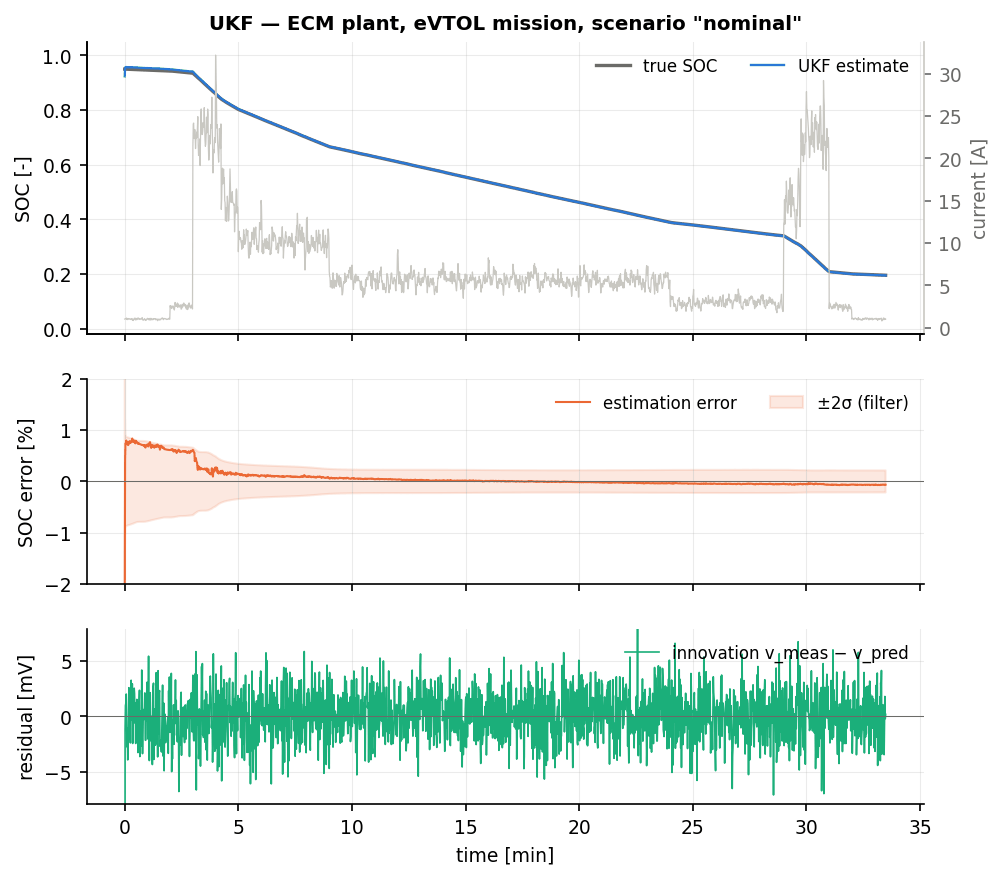
\includegraphics[width=\textwidth]{figures/cell_UKF_nominal.png}
\caption{UKF on the nominal eVTOL mission: true and estimated SOC (top), estimation error with the $\pm 2\sigma$ band when available (middle), voltage residual (bottom).}
\end{figure}
\begin{figure}[H]\centering
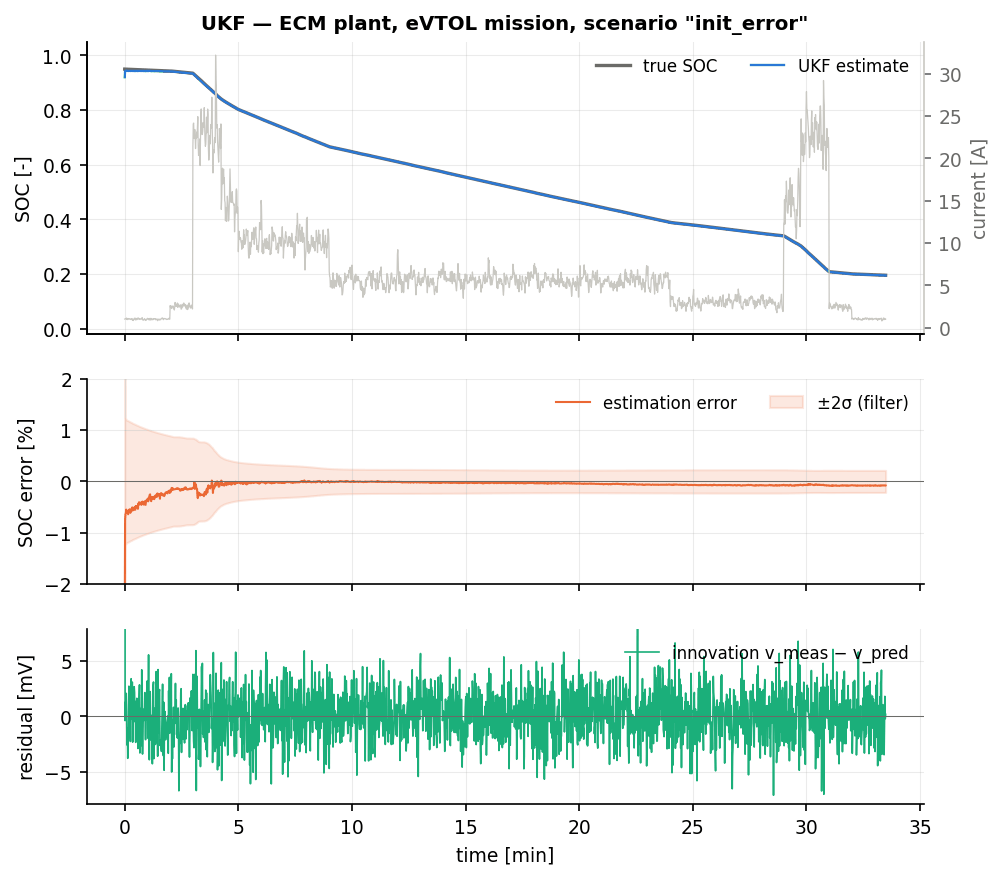
\includegraphics[width=\textwidth]{figures/cell_UKF_init_error.png}
\caption{UKF with a 35\,\% initial SOC error.}
\end{figure}
\begin{figure}[H]\centering
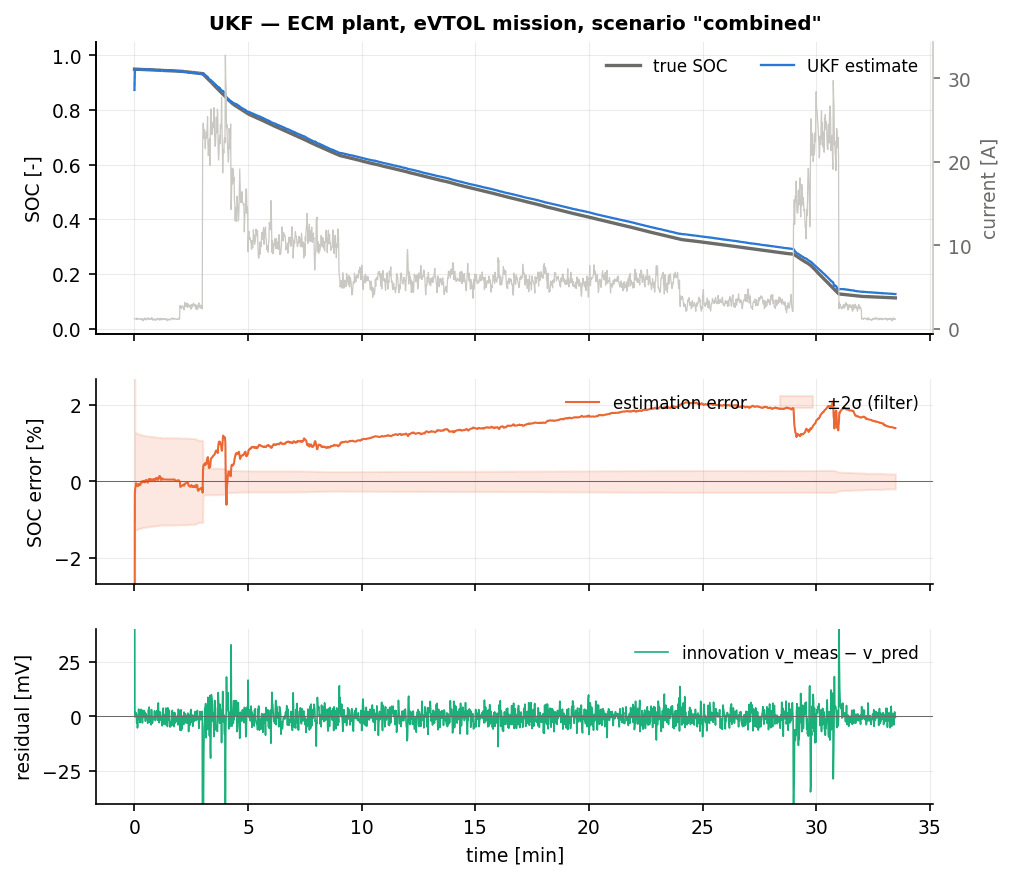
\includegraphics[width=\textwidth]{figures/cell_UKF_combined.png}
\caption{UKF on the \texttt{combined} scenario: the inflated predicted-measurement variance keeps the gain alive and the estimate locks onto the truth within seconds, where the EKF never recovers.}
\end{figure}

All numbers are three-seed means in per cent SOC.

Nominal performance is marginally better than the EKF's in steady state
($\text{RMSE}_{\text{ss}} = 0.04\,\%$ against $0.05\,\%$) but worse over the whole run
($0.20\,\%$ against $0.15\,\%$), with a maximum error of $4.02\,\%$ against $1.07\,\%$. Both
come from the same place: the transient of the first few seconds, where $\mP$ is still at its
initial value and the second-order term of Remark~\ref{rm:ukf-w0} makes the filter deliberately
cautious. With the $-35\,\%$ initial error the caution costs a little
($0.07\,\%$ steady state against the EKF's $0.05\,\%$) but both converge in the first sample.

The decisive result is \texttt{combined}, where the EKF reaches
$\text{RMSE}_{\text{ss}} = 12.44\,\%$ and never converges while the UKF reaches $1.19\,\%$ and
converges immediately --- the best figure of all fifteen filters on that scenario, marginally
ahead of the second-order EKF ($1.28\,\%$) and the IPLF ($1.72\,\%$). The state trace explains
it completely: after the first update the EKF reports $\sigma_\soc = 0.0065$ and the UKF
$\sigma_\soc = 0.0416$; $20$\,s later the UKF has pulled the estimate onto the truth
($0.9488$ against a true $0.9488$) whereas the EKF is stuck at $0.852$ and stays wrong for the
rest of the flight. The extra variance in $\mP_{yy}$ --- a genuine second-order effect, not a
fudge factor --- is what keeps the gain alive long enough to find the right answer. Note
however that this is an \emph{indirect} benefit of $\alpha = 0.1$: the same inflation appears
explicitly and more cheaply in the second-order EKF (Chapter~\ref{ch:soekf}).

Elsewhere the UKF and the EKF are close, with the UKF ahead on the scenarios where extra
caution helps --- \texttt{cold} $0.07\,\%$ against $0.16\,\%$, \texttt{aged\_cell} $1.36\,\%$
against $1.52\,\%$, \texttt{outliers} $0.18\,\%$ against $0.21\,\%$ --- and behind where it does
not: \texttt{sensor\_dropout} $0.86\,\%$ against $0.46\,\%$ and \texttt{preisach} $0.23\,\%$
against $0.20\,\%$ with a convergence time of $214$\,s against $16$\,s. The
\texttt{preisach} scenario changed character when the plant's hysteresis sign convention was
corrected: it is now a mild $0.2\,\%$ bias for the whole family rather than a differentiator,
and what the UKF loses there is convergence speed, not accuracy.

\paragraph{SPM plant: structured model error.}
\begin{figure}[H]\centering
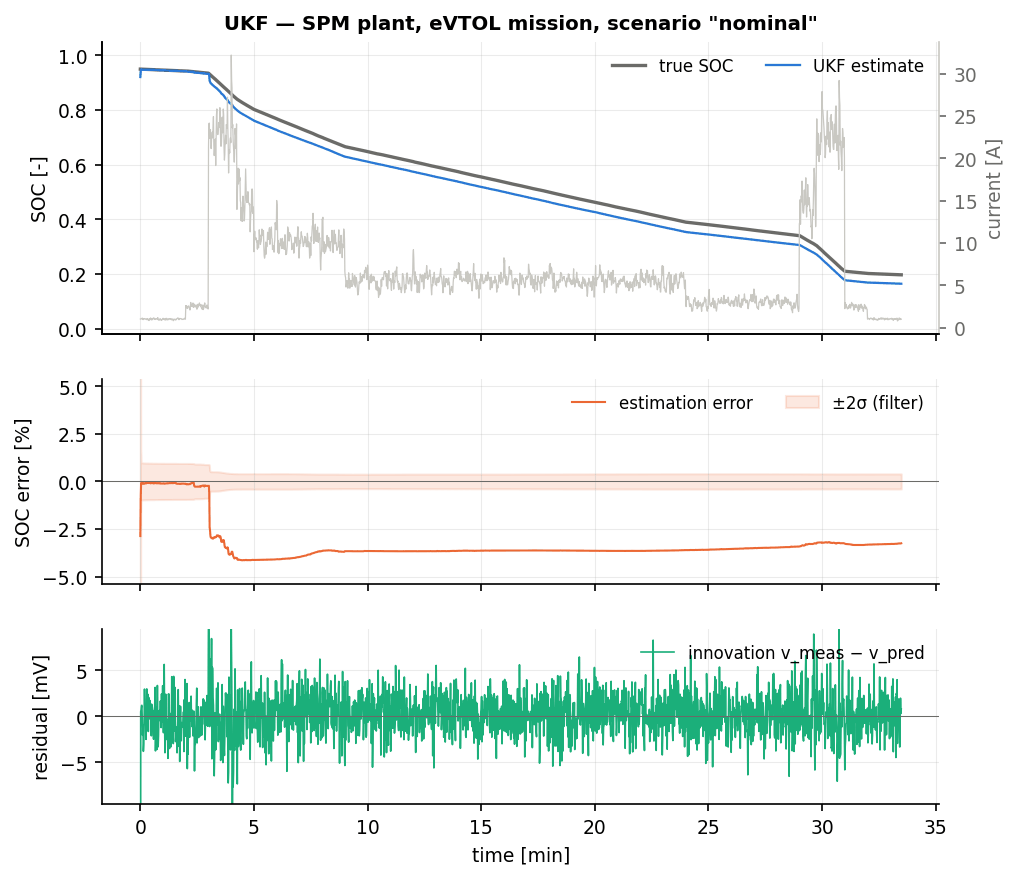
\includegraphics[width=\textwidth]{figures/cellspm_UKF_nominal.png}
\caption{UKF on the nominal mission with the electrochemical (SPM) plant.}
\end{figure}
The SPM block of the table is a different kind of test. The plant is the electrochemical
single-particle model; the estimator still runs a 2-RC equivalent circuit, fitted to that plant,
which leaves a \emph{structured} residual of about $4$\,mV (Butler--Volmer kinetics and
solid-phase diffusion that no 2-RC circuit can reproduce) and a slow second branch,
$\tau_2 = 556$\,s. Over a $33$-minute mission a $556$\,s pole barely relaxes, so $v_2(t)$ is
close to an affine ramp --- and so is $\ocv(\soc(t))$ while the cell discharges at a roughly
constant rate. The two channels through which the measurement sees the state,
$(\partial\ocv/\partial\soc)\,\delta\soc$ and $-\delta v_2$, are therefore nearly collinear in
the information accumulated over the flight: the pair $(\soc, v_2)$ is close to unobservable,
and no filter can decide whether a persistent few-millivolt residual belongs to the slow RC
branch or to the state of charge. Because that direction is weakly observable, a $4$\,mV
structured error maps onto \emph{several per cent} of SOC instead of the
$4\,\text{mV}/0.8\,\text{V}\approx0.5\,\%$ a well-conditioned channel would give. This
$(\soc,v_2)$ ambiguity, not the size of the residual, is the mechanism behind the
$3.7$--$4.6\,\%$ band in which the whole classical family sits.

The UKF sits at $3.96\,\%$ on SPM \texttt{nominal}, slightly \emph{worse} than the EKF's
$3.73\,\%$, and the gap widens on the harder rows: \texttt{cold} $8.29\,\%$ against $7.35\,\%$,
\texttt{param\_mismatch} $4.95\,\%$ against $3.13\,\%$, \texttt{sensor\_dropout} $7.26\,\%$
against $5.31\,\%$. This reverses the ECM ordering and it follows directly from the ambiguity
argument: the unscented transform performs a statistical regression of $h$ over the prior, and
a regression puts \emph{more} weight on the OCV channel than a tangent does, so it commits
harder to the direction that carries the structured error. The exception is
\texttt{outliers}, where the UKF's extra caution again pays ($1.76\,\%$ against $1.99\,\%$).
The general lesson is worth stating: better moment propagation is a remedy for nonlinearity,
not for a model that is structurally wrong, and on the SPM plant it is mildly
counter-productive.

\section{Summary}
The UKF costs about three times an EKF step and buys derivative-free implementation plus
second-order accurate moments. On this cell model that is worth little in most ECM scenarios
--- the dynamics are affine and the prior is usually tight --- and worth everything in the one
scenario where a large prior meets the curved OCV characteristic, where it is the best filter
of the fifteen. Choose it when Jacobians are unavailable or unreliable, when the initial SOC
uncertainty is large (first power-up, after a pack swap), or when the same filter must also
carry parameters. Do not expect it to fix biased sensors, a wrong capacity, or structured model
error: on the SPM plant it is slightly worse than the plain EKF.
